\documentclass{article}
\usepackage{amsmath}
\usepackage{fancyhdr}
\usepackage{subcaption}
\usepackage{listings}
\usepackage{subcaption}
\usepackage{graphicx}
\usepackage[margin=1.5in]{geometry}
%command for creating spaces
\newcommand\tab[1][0.5cm]{\hspace*{#1}}
\title{\textbf{NEA}}
\author{Name: Jez Snelson\\
        Candidate Number: 1209\\
        Centre Number: 62337}
%Footer and Header
\fancyhead[L]{Title}
\fancyhead[R]{Oxford Spires Academy, Center No. 62337}
\fancyfoot[L]{Jez Snelson, Candidate No. 1209}
%Margins
\setlength{\marginparwidth}{0pt}
\begin{document}
\pagenumbering{roman}
\date{}
\pagestyle{empty}
\maketitle
\newpage
\tableofcontents
\newpage
\pagestyle{fancy}
\pagenumbering{arabic}
\section{Analysis}
        \subsection{The Problem}
        Dungeon Crawler style games can be boring and repetitive, this means they can have little to none replay value. Additionaly alot of Dungeon crawlers have a steep learning curve that makes it hard for new or casual players to fully enjoy them.\\
        \subsection{Client Request}
        The client has requested a Dungeon Crawler style game that has very good replay value whilst also being easy to learn and play casually.\\
        \newpage
        \subsection{Research}
        \subsubsection{Existing Solutions}
        \textbf{Edmund McMillen's The Binding of Isaac}\\
        Edmund McMillen created the popular dungeon crawler roguelike The Binding of Isaac and released it on Steam (https://store.steampowered.com/app/113200/The\_Binding\_of\_Isaac/).\\
        This game was relatively unique as it had procedurally generated dungeons \\using a system of rooms that tesalate with each other.\\
        \\
        The procedurally generated dungeons consist of different shaped square based rooms that tesalate and are generated next to each other in a psuedo random fashion whilst obeying a set of rules. The mobs that spawn in each room can vary but there is usually only one or two enemy types per room and as you go up levels the amount of enemies and difficulty the pose increases. This system allows for every playthrough of the game to be different to the next with the same reccuring theme/difficulty which allows for lots of replay oppurtunity.\\
        \\
        However, the game has a couple issues that mean that it does not completely solve our problem. First is the steep learning curve that the game presents which, although to some is a welcome challenge, can put off new or less experienced players especially due to its roguelike nature meaning when you die you start from scratch. The game also has an unintuitive movement and fighting system as there is only really quad directional projectiles and a simple walking design which when combined contributes to the steep learning curve.\\
        \begin{figure}[h]
                \centering
                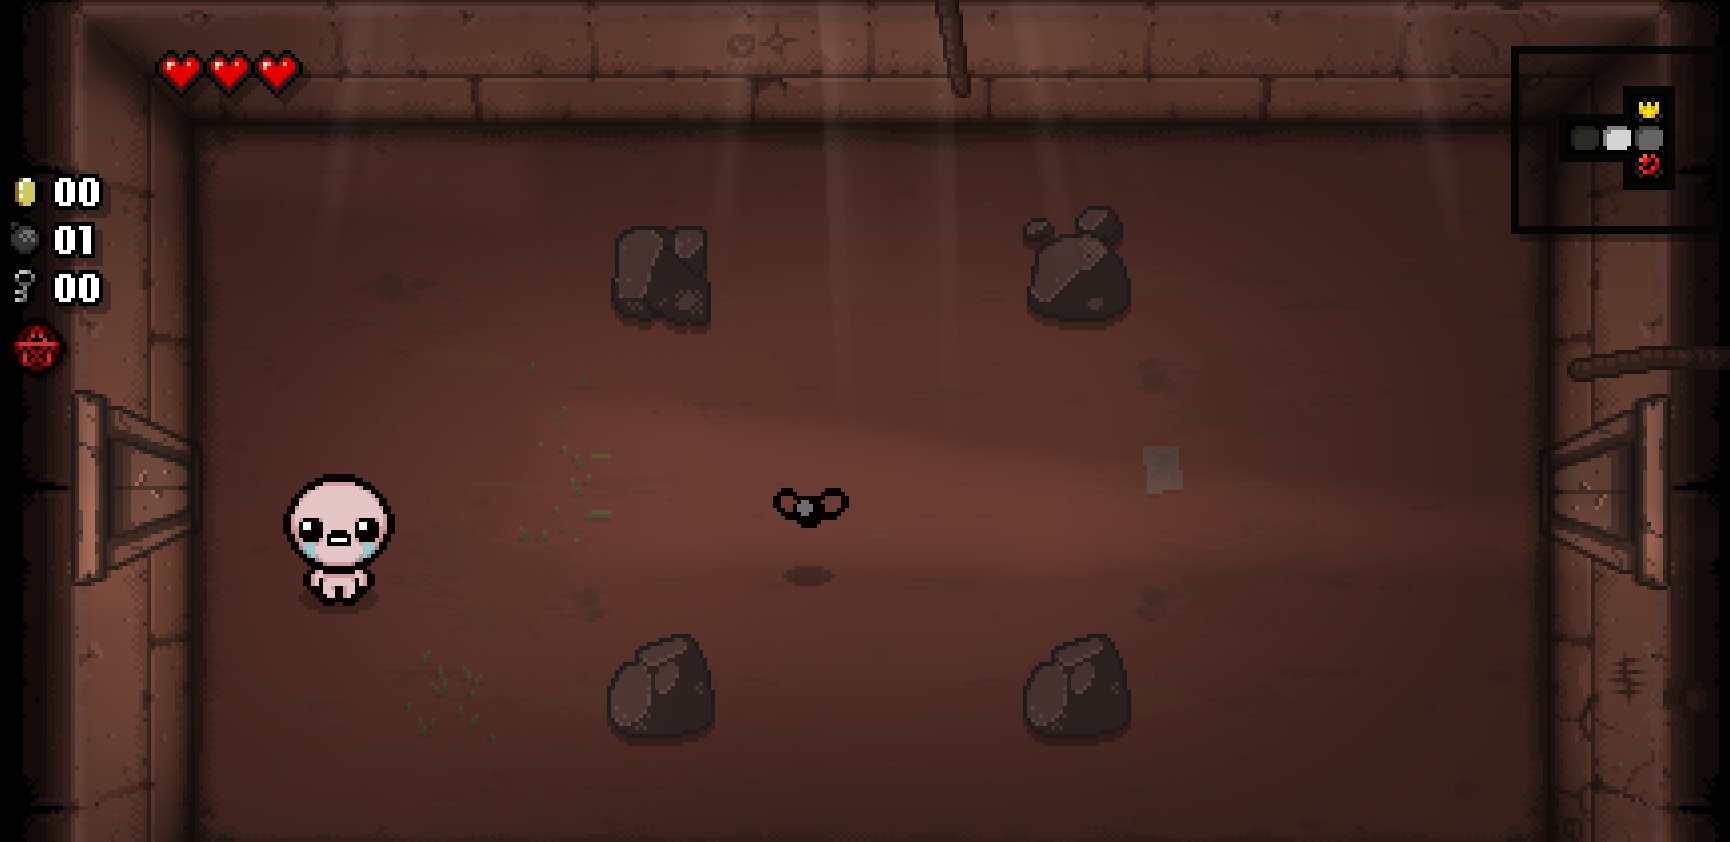
\includegraphics[scale=0.25]{images/research/BOI_Capture.PNG}
                \caption{A screenshot of The Binding of Isaac}
                \label{fig:ie_0}
        \end{figure}
\newpage
\pagestyle{plain}
\section{References}
\end{document}